\subsection{Chapter Overview}

\subsection{The Bayesian Formulation of Predictions}

As stated in chapter one and two, the quantification of uncertainty provides additional value in monitoring machine energy performance and evaluating whether or not a machine is deviating from the expected behavior. Motivated by this, the Bayesian framework will be used as uncertainty quantification is a central component, and as a result, we will have access to probability distributions over predictions instead of point predictions.

Why do we have access to uncertainty?
 - Prior, likelihood, posterior
 

\subsection{Definition and Characteristics of Time Series}

A time series is a sequential set of data points indexed by time $t$ with some output $y$. It is typically defined as a set of vectors $y(t), t = 0, 1, 2,. . .,n$ where $t$ represents the time elapsed and $y$ is the output. A time series is \textit{univariate} if it consists of single observations recorded over equal periods of time. For example, monthly CO2 measurements is a \textit{univariate} time series. Furthermore, more variables may be added to a time series to make it \textit{multivariate}. A \textit{multivariate} time series consists of multiple time-dependent variables where each variable may also have some dependency on other the variables. Time series can also be discrete or continuous. Continuous time series are recorded at every instance of time, even when the measured variable can only take a discrete set of values (company sales, number of unemployed persons). Discrete time series are when observations are taken only at specific times, usually equally spaced, even if the measured variable is a continuous variable. In this thesis, a continuous time series is discretized by aggregating the time series into equally spaced intervals of 10 and 30 minutes upon which the continuous variable (Watts) is analyzed. 

Within a time series, there are typically four components to be considered which may influence the analysis or modeling. Not all time series contain all four components, and certain models are aimed at modeling time series with only a subset of these components. Thus, the exploratory data analysis (EDA) and subsequent model selection are important phases of time series analysis. Below, the main components of a time series are defined.

\textbf{Trend}: A trend is a general tendency of a time series to increase, decrease or stagnate over time \cite{tsa}. For example, global warming, a time series referring to the global temperature, exhibits an increasing trend. 

\textbf{Seasonal}: Seasonality is when a time series is influenced by seasonal factors (e.g., the quarter of the year, the month, or day of the week). Time series longer in duration may have multiple seasonality components. For example, airline data on the number of passengers flying exhibits multiple seasonality—vacation and holiday periods \cite{tsa}.

\textbf{Cyclical}: The cyclical variation in a time series describes data that exhibits rises and falls that are \textit{not of fixed period}. The duration of a cycle depends on the type of industry or business being analyzed. For example, electrical load profiles of residential buildings often exhibit a cyclical pattern as the demand for energy \textit{cycles} throughout the day, but is typically not of a fixed period, i.e., people continue living in the building for a long period of time. 

\textbf{Irregular}: This component is unpredictable. Every time series has some unpredictable component that makes it a random variable. In prediction, the objective is to “model” all the components to the point that the only component that remains unexplained is the random component. This component is also sometimes called the \textit{residual} \cite{tsa}. 

In this thesis, it is expected that the industrial equipment will show a strong cyclical pattern as the loads of the equipment will be influenced by production process schedules; in turn influenced by the "business week". In \hyperlink{subsection.4.2}{section 4.2}, an exploratory analysis will be conducted to visualize the components of the machine's time series. 


\subsection{Introduction to Gaussian Processes for Time Series}

Gaussian Processes (GPs) belong to the family of \textit{Bayesian non-parametric models} and offer a principled, interpretable, and intuitively specified way for conducting probabilistic inference of non-linear time series. Non-parametric methods do not assume a fixed parametric form for the prediction function, but instead try to estimate the function itself (rather than the parameters) directly from the data. 

GPs can be viewed as a generalization of a Gaussian distribution in $\mathbb{R^n}$ to a space of functions. More specifically, a GP is a way to define distributions over functions with the assumption that the function values at a set of $M > 0$ inputs, $f = [f(x_1), . . .,f(x_M)]$, is jointly Gaussian with a mean $(\mu = m(x_1), . . .,m(x_M))$ and covariance $\sum_{i, j} = K(x_i, x_j)$, where $m$ is the mean function and $K$ is a positive definite kernel. A positive definite kernel is a generalization of a positive definite matrix where the matrix is symmetric and all its eigenvalues are positive. 

Thus, the two central components of a GP are the mean $m(x)$ and covariance kernel function $k(x_i, x_j)$. The former represents the value we expect for our function before seeing the data, and the latter, the beating heart of a GP, specifies the correlation between any pair of outputs and therefore determines the properties of the function that it generates. The kernel allows one to encode prior knowledge about the similarity of the two input vectors $x_i$ and $x_j$, i.e., if we know that $x_i$ is similar to $x_j$, then the model can be encouraged to make the predicted output at both locations $f(x_i)$ and $f(x_j)$ to be similar. As the problem in this thesis is concerned with time series, the informativeness of past observations in explaining current data is a function of how long ago the past observations were observed. The covariance matrix for a set of locations $x = \{x_1, x_2, . . .,x_n\}$ is defined as:

\begin{equation}
\mathbb{K(x, x') = \begin{pmatrix}
k(x_1, x_1) & k(x_1, x_2) & \dots & k(x_1, x_n) \\
k(x_2, x_1) & k(x_2, x_2) & \dots & k(x_2, x_n) \\
\vdots & \vdots & \vdots & \vdots \\
k(x_n, x_1) & k(x_n, x_2) & \dots & k(x_n, x_n)
\end{pmatrix}}
\end{equation}

This means that the entire function evaluation, associated with points in $x$, is drawn from a multivariate Gaussian distribution:

\begin{equation}
p(y(x)) \sim \mathcal{N}(m(x), K(x, x'))
\end{equation}

where $y = \{y_1, y_2,. . .,y_n\}$ are the dependent function values, evaluated at locations $x_1,. . .,x_n$, $m$ is a \textit{mean function} and $K$ is a kernel function, again evaluated at the locations of the $x$ variables. If one believes there is noise (which there often is) associated with the observed function values $y_i$, then a noise term can be directly incorporated into the covariance function:

\begin{equation}
K(x, x') + \sigma^2I
\end{equation}

where $I$ is the identity matrix since noise is expected to be uncorrelated from sample to sample; hence noise only needs to be added to the diagonal of $K$. The $\sigma^2$ is a hyper-parameter representing the noise variance.

A GP with a given \textit{mean function} $m$ and \textit{covariance function} $K$ is a prior that can generate functions; hence the common definition of a GP as "a prior distribution over functions". Now that the central components of a GP have been laid out, the following describes how to perform inference. To perform inference with GPs from some input (test data) $x_*$ given some training data $D = \{(x_i, y_i)\}$ assuming i.i.d additive Gaussian noise with variance $\sigma_{n}^2$, the prediction and observations are expressed as a joint distribution following the GP prior:

\begin{equation}
\begin{bmatrix} 
y \\ 
y_*
\end{bmatrix} 
\sim{~} \mathcal{N} (m, \begin{bmatrix} 
K(X, X) + \sigma_{n}^2I & K(X, X_*) \\
K(X_*, X) & K(X_*, X_*)
\end{bmatrix})
\end{equation}

where $y_*$ is some output test data and $X_*$ is the input test points. One can think of the evaluation of test points $X_*$ at new locations as \textit{augmenting} the observed data $X$ with the test data $X_*$ and $y_*$ in the joint distribution. 

With the product rule, one can relate the joint distribution to the conditional distribution to obtain the posterior predictive distribution given by:

\begin{equation}
p(f_* | X_*, X, y) = \mathcal{N}(f_* | m_*, \sum_*)
\end{equation}

with mean and covariance given by:

\begin{equation}
m^* = m(x_*) + K(X_*, x)(K(X, X) + \sigma_{n}^2)^{-1}(y - m(x))
\end{equation}
\begin{equation}
\sum_{*} = K(X_*, X_*) - K(X_*, x)[K(X, X) + \sigma_{n}^2]^{-1}K(X, X_*)
\end{equation}

Gaussian Process models have a number of parameters $\theta$ (sometimes called hyperparameters) resulting from the mean and kernel function that must be \textit{marginalized} in order to perform inference. As a GP is within the Bayesian framework, priors are first assigned to these hyperparameters using distributions utilizing our domain knowledge. Kernel parameters and incorporating expert opinion through the use of the auto-correlation function (ACF) is described in \hyperlink{subsection.3.5}{section 3.5}. Ideally, with prior distributions assigned to the hyperparameters, we would like to use Bayes rule to compute the posterior to find the \textit{most likely} parameters:

\begin{equation}
p(\theta | y) = \frac{p(y | \theta)p(y)}{p(y)}
\end{equation}

However, the marginal likelihood $p(y | \theta)$ is almost always intractable and we must therefore use approximation techniques. To find the \textit{most likely} hyperparameters, the marginal log-likelihood is maximized through gradient-based optimization and is given by the form:

\begin{equation}
log P(y | X, \theta) = -\frac{1}{2}y^T(K_{y} + \sigma_{n}^2)^{-1} - \frac{1}{2}log|K_{y} + \sigma_{n}^2| - \frac{n}{2} log(2\pi)
\end{equation}

In \hyperlink{subsection.5.2}{section 5.2}, the experimentation setup pertaining to the type of optimizer used, number of training iterations, and learning rate is given. Although the above is technical, GPs have an intuitive procedure for training and performing inference: encode prior beliefs with kernels $\rightarrow$ condition on what you have observed $\rightarrow$ optimizer parameters $\rightarrow$ use posterior predictive distribution for performing inference.

\subsection{Covariance and Mean Functions}

As outlined above, the kernel design is a vital step in GP model design and offers an opportunity to incorporate domain knowledge into the model. Below, a few kernels and their hyperparameters that will be useful in modeling non-linear time series will be introduced and subsequently, an explanation on how to compose kernels through addition or multiplication will be provided.

\subsubsection{Squared Exponential Kernel}

First, the \textit{squared exponential} or \textit{radial basis function} ($RBF$) kernel is one of the most widely used kernels for real-valued inputs. Notably, the $RBF$ is a stationary kernel that encodes a high degree of smoothness in the function space, and hence can be used to design a GP which produces functions that can be smooth,

\begin{equation}
    K_{RBF} = \sigma^2 exp(-\frac{||x - x'||}{2 \ell^2})
\end{equation}

where $\ell$ is the lengthscale and controls the "wiggliness" of the function and $\sigma^2$ is the overall variance / outputscale  ($\sigma$ is also known as the amplitude) of the function. In \hyperlink{figure.1}{Figure 1} below, three functions are sampled and visualized from an RBF kernel; each with different length and outputscale values.

\begin{figure}[htp]
\centering
\graphicspath{ {./images/} }
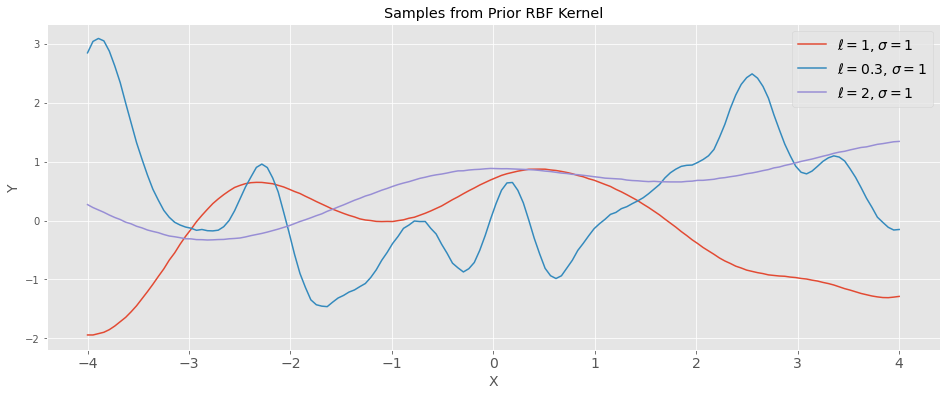
\includegraphics[scale=0.49]{images/samples_rbf_prior.png}
\caption{Three samples, each from an $RBF$ kernel with different hyperparameters denoted by the table legend. Notice how $\ell$ affects the smoothness of the function.}
\end{figure}

\subsubsection{Periodic Kernel}

The \textit{periodic} ($Per$) kernel captures repeating structures, which can model seasonalities influenced by business cycles and or human behavior. For example, home electricity consumption often displays daily seasonalities. The \textit{periodic} kernel has the form

\begin{equation}
K_{per} = exp(-\frac{2}{\ell^2} sin^2 (\pi \frac{r}{p}))
\end{equation}

where $p$ is the period. Again, $\ell$ and $\sigma^2$ are the lengthscale and outputscale respectively. \hyperlink{figure.2}{Figure 2} below visualizes the repeating structures of the $Per$ kernel. Important in this thesis is how the period is chosen. In a time series, the correlation between any pair of outputs can be analyzed empirically using the autocorrelation function (ACF). The ACF compares the time series with itself at a certain lag. Namely:

\begin{figure}[htp]
\centering
\graphicspath{ {./images/} }
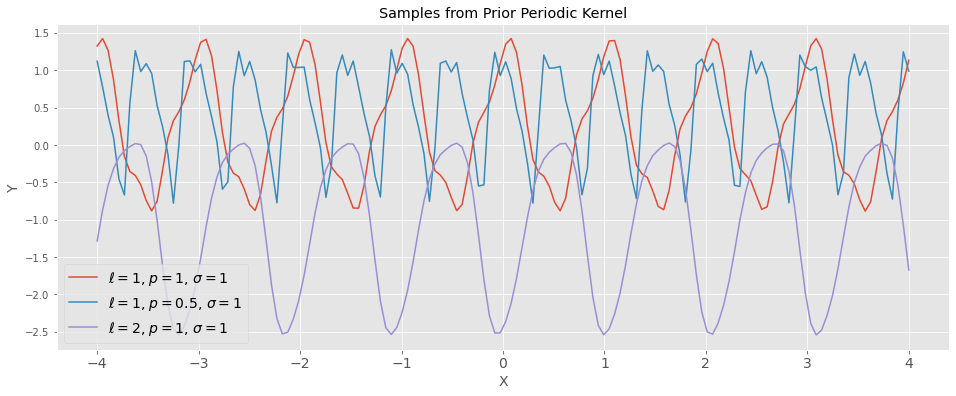
\includegraphics[scale=0.49]{images/samples_periodic_prior.png}
\caption{Three samples, each from a $Per$ kernel with different hyperparameters denoted by the table legend. Notice how $p$ affects the periodicity of the function and $\ell$ affects the "wiggliness" of the variations.}
\end{figure}

\begin{equation}
    \hat{p}(k) = \frac{\sum_{s=1}^{n-k}(x_{s+k} - \bar{x})(x_s - \bar{x})}{\sum_{t=1}^{n-k}(x_t - \bar{x})^2} 
\end{equation}

Thus, using the ACF coefficients, the interval of periods that show significant autocorrelations are chosen as the prior belief for the time series cyclical period length. Increasing the period $p$ increases the distance between repetitions. \hyperlink{figure.3}{Figure 3} below shows an example of the ACF correlogram for the paper disposal machine and how one can use the coefficients at certain lags as a prior belief for modeling the cyclical component. 

\begin{figure}[htp]
\centering
\graphicspath{ {./images/} }
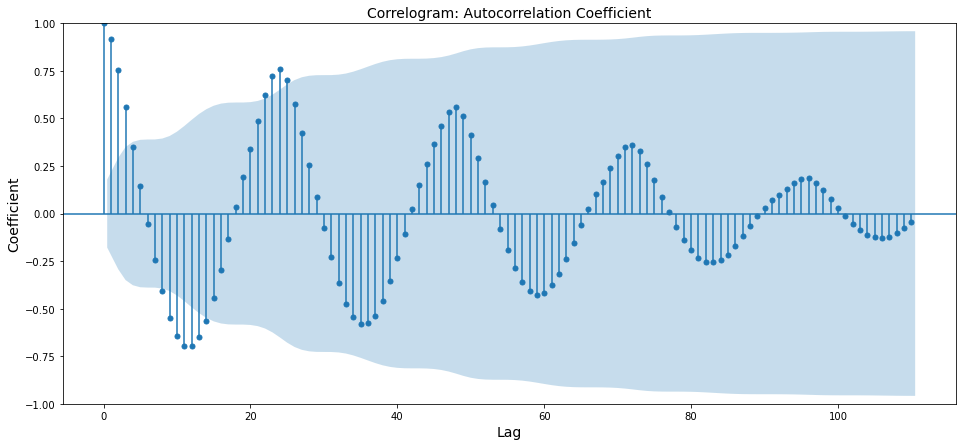
\includegraphics[scale=0.49]{images/entsorgung_acf.png}
\caption{Entsorgung ACF. The time series is discretized and averaged at 1hr intervals. Therefore, the ACF shows significant autocorrelations between $10$ and $12$ hours and $22$ and $24$ hours with the remaining lags decreasing in amplitude and significance.}
\end{figure}

\subsubsection{Rational Quadratic Kernel}

The \textit{Rational Quadratic} ($RQ$) kernel can be interpreted as the sum of many $RBF$ kernels of different lengthscales. Similar to the $RBF$, the $RQ$ kernel encodes smoothness in the function space, but with the additional flexibility of having both local variations and long term variations. 
\begin{equation}
    K_{RQ} = \sigma^2 exp(1 + \frac{(x - x')^2}{2\alpha \ell^2})
\end{equation}

where $\alpha$, also known as the scale mixture, determines how much local variations from the smaller lengthscales contribute to the overall variation. By using this kernel, one can model non-periodic trends of the underlying physical process and interpret the hyperparameters $\ell$ as either a non-periodic hourly or daily trend depending on how large or small the value of $\ell$ is respectively. Three samples of the RQ kernel are visualized in \hyperlink{figure.4}{Figure 4}.

\begin{figure}[htp]
\centering
\graphicspath{ {./images/} }
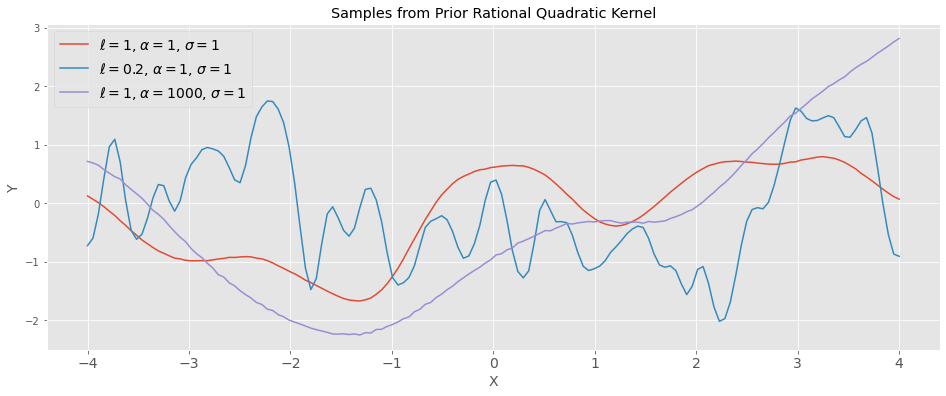
\includegraphics[scale=0.49]{images/samples_rq_prior.png}
\caption{Three samples, each from a $RQ$ kernel with different hyperparameters denoted by the table legend. Notice how $\alpha$ affects the . . . of the function and $\ell$ affects the "wiggliness" of the variations.}
\end{figure}

\subsubsection{Kernel Composition}

Kernels can also be combined through addition and multiplication given the result is a positive definite kernel. Therefore, by combining kernels, more complex covariance structures can be designed. The addition of two kernels $K_1(x, x')$ and $K_2(x, x')$ is analogous to the probabilistic "OR" operation, i.e., two points $x_1$ and $x_2$ are considered highly correlated if they are highly correlated in $K_1 \lor K_2$. The multiplication of the two kernels is analogous to the probabilistic "AND" operation, i.e,. two points $x_1$ and $x_2$ are considered highly correlated if they are highly correlated in $K_1 \land K_2$. The resulting kernel given by the addition or multiplication of the two kernels is given by:

\begin{equation}
    K(x, x') = K_1(x, x') + K_2(x, x')
\end{equation}
\begin{equation}
    K(x, x') = K_1(x, x') * K_2(x, x')
\end{equation}

\subsubsection{Locally Periodic Kernel}

In time series analysis, the periodic structure of the underlying function may change and or may not be consistent over time. For example, \textbf{figure #} shows a daily repeating cycle that changes its structure over the course of the week. Thus, one may want to incorporate this locally changing periodic structure "belief" into the kernel design. To do this, a \textit{locally periodic kernel} ($LocPer$) is introduced. The $LocPer$ kernel is a product of the $K_{RBF}$ and $K_{Per}$:

\begin{equation}
    K_{LocPer} = \sigma^2 exp (-\frac{2sin^2(\pi(x - x') / p}{\ell_{Per}^2}exp(-\frac{(x - x')^2}{\ell_{RBF}^2}))
\end{equation}

The periodic component correlates points that are far away from each other, but still in the same phase of a cycle. The $K_{RBF}$ decorrelates the two points and how quickly the points are decorrelated is determined by the hyperparameter $\ell_{RBF}$. Remember, $ell_{RBF}$ determines the "wiggliness" of the function; therefore smaller $\ell_{RBF}$ corresponds to faster changing periodic cycles and vice versa. The $K_{LocPer}$ is of use in modeling industrial machine equipment energy consumption as production processes are typically influenced by human behavior. Below, in \hyperlink{figure.5}{Figure 5}, three samples are generated from a $LocPer$ kernel.

\begin{figure}[htp]
\centering
\graphicspath{ {./images/} }
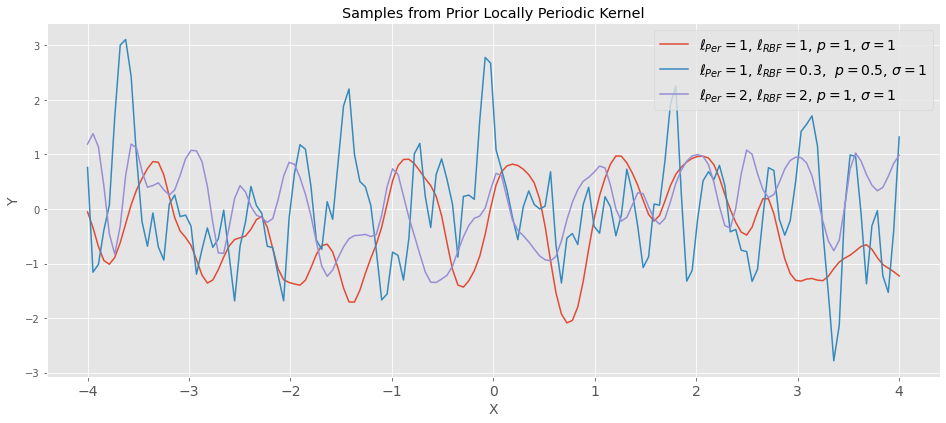
\includegraphics[scale=0.49]{images/samples_locper_prior.png}
\caption{Three samples, each from a $LocPer$ kernel with different hyperparameters denoted by the table legend. Notice how the product of the two kernels results in a periodic structure with variations in each cycle.}
\end{figure}


\subsection{Advantages and Disadvantages of Gaussian Processes}

In this thesis, Gaussian Processes for time series was chosen as a principled way to: 1.) perform probabilistic inference, 2.) allow for an intuitive model interpretation by way of \textit{decomposition} of the kernels, and 3.) incorporate background information in the form of \textit{kernel design}. 

However, GPs also have disadvantages. Here, a couple of the main challenges are presented relating to use in Industry 4.0. First, GPs. . .

\subsection{Evaluation Metrics}

To evaluate the performance of the model, the data set is first split into training and testing sets. The training set consists of four days of data where as the testing set consists of one days (24 hours) worth of data. Then, as GPs are probabilistic models, to evaluate model quality, not only should the accuracy of the model's predictions be computed, but also how precise the predictions are using the posterior predictive distribution. Thus, deterministic and probabilistic error metrics are used in this thesis. The following metrics are used to evaluate the performance and quality of the model: Mean Squared Error (MSE), Root Mean Squared Error (RMSE), Mean Absolute Percentage Error (MAPE), Average Coverage Error (ACE), and Pinball Loss.

\begin{itemize}
    \item \textit{MSE}: Also known as the average squared loss, measures the average squared distance the predictions are from the actual values. A larger MSE indicates that the data points are dispersed more widely around the mean, whereas a smaller MSE suggests the inverse. In regression, the smaller the MSE, the better. MSE is given by:
    
    $$\frac{1}{n}\sum_{i=1}^n(\hat{y} - y)^2$$
    
    \item \textit{RMSE}: Is the square root of MSE. The square root function turns the metric back into the same units as the dependent variable $y$. Again, the smaller the RMSE, the better and is defined as :
    
    $$\sqrt{\frac{1}{n}\sum_{i=1}^n(\hat{y} - y)^2}$$
    
    \item \textit{MAPE}: Measures the accuracy of the forecast as a percentage and offers an intuitive way to communicate the quality of a model to non-technical audiences. For example,  a $15\%$ MAPE would mean that, on average, the model is off the true value by $15\%$. The smaller the MAPE, the better, and is defined as:
    
    $$\frac{1}{n}\sum_{i=1}^n \frac{|A_t - F_t|}{A_t}$$
    
    where $A_t$ is the actual value and $F_t$ is the forecasted value. The absolute difference is then divided by the actual value $A_t$ to obtain a scale-independent measure. 
    
    \item \textit{ACE}: Sampling functions from the posterior predictive distribution, one can obtain prediction intervals (PI). In this thesis, two standard deviations (95\%) is used. ACE measures the proportion of actual values within the PI and is bounded between $[0, 1]$:
    
    $$ I_t = 
    \begin{cases}
      1 & \text{if} \quad P_t \in [\hat{L_t}, \hat{U_t}] \\
      0 & \text{if} \quad P_t \notin [\hat{L_t}, \hat{U_t}]
    \end{cases}
    $$
    $$UC = \frac{1}{|T|}\sum_{t\inT}I_t$$
    
    where $P_t$ is the actual value at time $t$, and $I_t$ is a binary indicator of whether the PI $ [\hat{L_t}, \hat{U_t}]$ contains $P_t$. Since ACE measures a proportion of the actual values contained by the PI, this proportion measures the discrepancy between the percentage of points contained by the PI and the confidence level (CI) of the PI; here two standard deviations represents a 95\% CI. However, ACE can be misleading due to the fact that a wide PI can cover all the actual data points—resulting in a high score. Therefore, ACE is complemented by the Pinball loss.
    
    \item \textit{Pinball Loss}: Measures the sharpness of the PI which evaluates the precision of the prediction and how sharp (or tight) the PI is around the actual value. Pinball loss is defined as:
    
    $$ \text{Pinball}(q, t) = 
    \begin{cases}
    (1 - q)(\hat{Q_t}(q) - P_t) \quad \text{for} \quad P_t < \hat{Q_t}(q) \\
    (q)(P_t - \hat{Q_t}(q)) \quad \text{for} \quad P_t \ge \hat{Q_t}(q) 
    \end{cases}
    $$
    
    where $\hat{Q_t}(q)$ is the predicted $q^{th}$ quantile at time $t$. The pinball loss is calculated at every time step $t$ and is then averaged. The final pinball loss metric is calculated by averaging the pinball loss for $99$ percentiles. Thus, what is desired, is a prediction with high ACE and a low Pinball loss which indicates a probabilistic prediction is accurate and with low uncertainty.
    
\end{itemize}

During the experimentation phase, as outlined in \hyperlink{subsection.5.2}{section 5.2}, different model and kernel designs were compared such that the better model was the one that minimized MSE, MAPE, RMSE, and Pinball loss, while subsequently maximizing ACE. Also, in this thesis, the metrics MSE, MAPE, and Pinball loss were computed using scikit-learn's \cite{scikit-learn} metric library. Furthermore, ACE and RMSE were calculated from scratch. 



